%INTRO
This chapter covers the theory needed to understand the implementation in chapter \ref{ch4}. 
It covers the Eclipse Arrowhead frame more in depth than chapter \ref{ch2} did.
This chapter covers how the Eclipse Arrowhead framework is built up and how the end user can interact with the framework in the best possible way.
The end of this chapter describes a test for measuring performance between the different IoT frameworks.
%AHF
\section{Eclipse Arrowhead framework} 
%Mandatory core systems.
As mentioned in the related work section, the Eclipse Arrowhead framework consists of three mandatory core systems
\begin{itemize}
    \item Service registry system.
    \item Authorization system. 
    \item Orchestration system.
\end{itemize} 
%Service registry system.
\subsection{Service registry system}
The service registry system is responsible for enabling discovery and registring services, Delsing et al. state. 
According to the Eclipse Arrowhead projects own GitHub page, the service registry system provides the database which stores the offered services in the local cloud.\cite{Github2021}
The Github page also states the three main objectives of the service registry system are:
\begin{itemize}
    \item To allow the application system to register available services to the database. 
    \item Remove or update available services from the database.
    \item Allow application system to use the lookup functionality of the registry.
\end{itemize}
%Authorization system.
\subsection{Authorization system}
According to the projects Github page, the Authorization system contains two databases for keeping track of which system can consume services from which other systems, depending on whether the Application system is in the same cloud or not.
The GitHub documentation also states that if the authorization happens within the same cloud, it is called intra-cloud authorization, and if it happens across two local clouds, it is called inter-cloud authorization.\cite{Github2021}
\subsection{Orchestrator system}
%Orchestrator system.
The Orchestration system is responsible for pairing and finding service providers and consumers, Delsing et al. declare.
Delsing et al. continue to state that the orchestrator also stores the orchestration requirements and the resulting orchestration rules.\cite{Delsing2017} 
The project's documentation argues that the main objective of the orchestrator system is to find an appropriate provider for the requesting consumer system.\cite{Github2021}

%Two types of orchestration
The documentation also states that there are two types of orchestration, store orchestration and dynamic orchestration.
Store orchestration uses the database orchestration store to find predefined orchestration rules.
On the other hand, dynamic orchestration searches the entire local cloud, or even other clouds, to find the matching provider.\cite{Github2021}
%AFHDB
\section{Arrowhead database}
%Intro
One can view the Eclipse Arrowhead framework as a series of database tables to connect.
%Clarification of tables.
One table relevant to all the core systems is the service\_interface table.
It correlates a connection interface, i.e., HTTP-INSECURE-JSON, HTTP-SECURE-JSON, and HTTPS-SECURE-JSON, to a specific ID used later on.
\subsection{Service registry system tables}
The tables in the Arrowhead database relevant to the service registry system are
\begin{itemize}
    \item system\_ keeps the information about consumers and providers. 
    \item service\_registry contains information about the different services.
    \item service\_definition, stores service definition name, and ID.
    \item service\_registry\_interface\_connection correlates a service registry ID to an interface ID.
\end{itemize}
\subsection{Authorization system tables}
The tables in the Arrowhead database relevant to the authorization system are
\begin{itemize}
    \item authorization\_intra\_cloud,  adds authorization rules for the provider, consumer, and service definition. Dictates which consumers are allowed to connect to which providers.  It also dictates the services the consumer is allowed to use.
    \item authorization\_intra\_cloud\_interface\_connection correlates an intracloud authorization ID to an interface ID.
\end{itemize}
\subsection{Orchestration system tables}
The tables in the Arrowhead database relevant to the orchestrator system are
\begin{itemize}
    \item orchestrator\_store,  contains orchestrator store entry, with information about which endpoints the consumers can use.
\end{itemize}

%SWAGGER
\section{Swagger UI}
The Eclipse Arrowhead framework has integrated Swagger UI into their core services. 
Meaning that the databases can be accessed and altered using HTTP methods instead of SQL queries.
Each core system has its swagger UI page, which serves as a visual, user-friendly REST API. 
A REST API, Representational state transfer, is a way to structure an API and consists of the following main principles according to Wikipedia.\cite{WIKIREST2021}
\begin{itemize}
    \item Each resource has its own URI.
    \item The resources have a common interface for commands between client and server. These are
    \begin{itemize}
        \item POST creates a new state for a resource.
        \item GET requests the state of a resource.
        \item PUT replaces the state of an already created state.
        \item DELETE deletes a resource state.
    \end{itemize}
\end{itemize}
Instead of sending SQL-queries, the Swagger UI uses JSON, JavaScript Object Notation, and how we should construct these will be covered in the implementation section.
%ARM MBED
\section{ARM Mbed}
%Intro
The  STM 32 board needs to be connected to the internet to use the Swagger UI. 
The ARM mbed OS 6 provides the functionality needed for this. 

%Foundations
Mbed OS 6 uses a hardware abstraction layer, HAL, to enable the microcontroller's most essential parts, such as timers.
When compiling your code,  libraries, drivers, and support for standard peripherals for microcontrollers are imported when using hardware supported by the Mbed OS 6.
This foundation enables the user to write applications against a shared set of APIs.
Another advantage of using supported hardware is the retargeting layer and boot process integration, so application development feels similar to C or C++ development.

%Connectivity
ARM Mbed OS enables the user to use a range of connectivity tools and suits. This thesis uses Wi-Fi, but there is support for Bluetooth, NFC, and much more on the STM32 B-L4S5I-IOT01A board.
Mbed OS connectivity and network stack offer a stable core of existing connectivity technologies, perfect for even the most demanding and versatile IoT applications. 

%Compilation - Expand this?
The Mbed online compiler allows the user to develop their code online, independent of the platform. 
The online compiler also supports the importation of code from GitHub, making it easier for the users to import this code and genuinely use this as a 'Getting started with the Eclipse Arrowhead framework' example. 


\section{Performance measurement}
Response time is measured to compare the performance of the three different IoT frameworks.  
Due to the vastly different implementation of the three frameworks, Amazon Web Services, Microsoft Azure, and Eclipse Arrowhead framework, the only thing worth measuring is the response time when pinging the different frameworks.

%Measurement
The Test-Connection command in power-shell sends four 32-bit packets to the specified destination. 
Iterating the Test-Connection 250 times gives us 1000 samples, a sufficient amount of attempts to produce an average response time.
The results from the Test-Connection is saved in a .csv file using the Export-Csv command. 
The Get-Content command then imports the saved data from the .csv file to keep all results through the whole loop.
\begin{figure}[H]
    \centering
    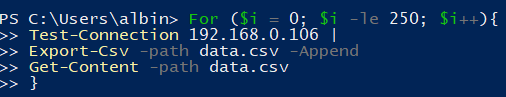
\includegraphics[width=\textwidth]{Pictures/powershell.png} 
    \caption{The powershell script for generating the test data.}
    \label{powershell}
\end{figure}

The average is calculated with
\begin{equation*}
    \text{average response time} = \frac{\sum \text{response times}}{\text{number of response times}}
\end{equation*} 
In addition to presenting the average response time, we will calculate the maximum and minimum response times to understand the different frameworks' performance further. 
The results of these calculations one can read in detail in chapter \ref{ch5}.



 
